\documentclass[ucs]{beamer}
\usepackage{polski}
\usepackage[utf8]{inputenc}
\usepackage{pgfplots}
\usepackage{tikz}
\usetikzlibrary{automata,positioning,shapes,shadows,arrows,backgrounds,trees,fit,calc,decorations.pathreplacing,decorations.markings}

\usetheme{Ilmenau}
%\usetheme{PaloAlto}

\title[Gas Analyzer]{Aplikacja systemu pomiarowego do analizy składu spalin opartego o sieć ELAN}
%\subtitle{Gas Analyzer}

\author[D. Karbowiak, G. Powała]{Mgr inż. Damian Karbowiak  \and Mgr inż. Grzegorz Powała}
\institute[Politechnika Śl.]{\large Politechnika Śląska \\\vspace{0.5cm} 
\includegraphics[height=0.3\textheight]{images/PolslLogo} }
\date{Gliwice, \today}
       
\setbeamertemplate{footline}[frame number]
\useoutertheme{infolines}
 
\begin{document}

\begin{frame}
  \titlepage
\end{frame}

\begin{frame}
\frametitle{Istota pomiarów}
\begin{itemize}
\setlength{\itemsep}{5pt}
\setlength{\parskip}{5pt}
\setlength{\parsep}{5pt}
\item Kontrola poprawności działania systemów pomiarowych zainstalowanych na obiekcie
\item Wyznaczenie kierunków modernizacji istniejących instalacji
\item Weryfikacja efektów przeprowadzonych modernizacji
\item Okresowa kontrola poprawności funkcjonowania obiektu - zgodność z obowiązującymi normami
\item Wspomaganie procesu projektowania i wdrażania prototypowych instalacji i rozwiązań
\end{itemize}
\end{frame}

\begin{frame}
\frametitle{Współpraca od lutego 2013}
\begin{center}
\begin{tabular}{cccccc}

\includegraphics[width=0.1\textwidth]{images/AEiILogo} &

\includegraphics[width=0.1\textwidth]{images/IILogo} &

\includegraphics[width=0.25\textwidth]{images/SKNIndustrumLogo} &

\includegraphics[width=0.1\textwidth]{images/WISiELogo} &

\includegraphics[width=0.1\textwidth]{images/IMIUELogo} &

\includegraphics[width=0.1\textwidth]{images/ZKiWPLogo} \\ 
\end{tabular} 
\end{center}

\begin{enumerate}
\setlength{\itemsep}{3pt}
\setlength{\parskip}{3pt}
\setlength{\parsep}{3pt}
\item Wydział Automatyki, Elektroniki i Informatyki
\begin{itemize}
\setlength{\itemsep}{3pt}
\setlength{\parskip}{3pt}
\setlength{\parsep}{3pt}
\item Instytut Informatyki
\begin{itemize}
\setlength{\itemsep}{3pt}
\setlength{\parskip}{3pt}
\setlength{\parsep}{3pt}
\item Koło Naukowe Przemysłowych Zastosowań Informatyki ,,Industrum''
\\ mgr inż. Damian Karbowiak
\\ mgr inż. Grzegorz Powała
\end{itemize}
\end{itemize}
\item  Wydział Inżynierii Środowiska i Energetyki
\begin{itemize}
\setlength{\itemsep}{3pt}
\setlength{\parskip}{3pt}
\setlength{\parsep}{3pt}
\item Instytut Maszyn i Urządzeń Energetycznych
\begin{itemize}
\setlength{\itemsep}{3pt}
\setlength{\parskip}{3pt}
\setlength{\parsep}{3pt}
\item Zakład Kotłów i Wytwornic Pary
\\ mgr inż. Tomasz Kress
\end{itemize}
\end{itemize}
\end{enumerate}
\end{frame}

%\begin{frame}
%\frametitle{Historia}
%\vspace{-2mm}
%\begin{itemize}
%\setlength{\itemsep}{0pt}
%\setlength{\parskip}{0pt}
%\setlength{\parsep}{0pt}
%\item \underline{22 luty 2013} \\
%Kontakt mailowy ze strony mgr inż. Tomasz Kress
%\item \underline{28 luty 2013} \\
%Pierwsze spotkanie w celu omówienia problemu i zadania
%\item \underline{21 marzec 2013} \\
%Wypożyczenie Ultramatu 23 i rozpoczęcie współpracy oraz realizacji projektu
%\item \underline{kwiecień -- czerwiec 2013} \\
%Realizacja projektu
%\item \underline{wrzesień 2013} \\
%Finalizacja pierwszej części i podstawowej wersji projektu
%\item \underline{23 październik 2013} \\
%Prezentacja na zebraniu Instytutu Maszyn i Urządzeń Energetycznych
%\item \underline{25 listopad 2013} \\
%Pierwsze testy w warunkach przemysłowych -- Elektrownia Ostrołęka
%\end{itemize}
%\end{frame}

\begin{frame}
\frametitle{Gas Analyzer - geneza}
\begin{enumerate}
\setlength{\itemsep}{5pt}
\setlength{\parskip}{5pt}
\setlength{\parsep}{5pt}
\item Realizacja pomiarów przemysłowych
\item Wykorzystywanie kilku analizatorów firmy Siemens
\item Zapisywanie pomiarów w tabelce na kartce
\item Ograniczona częstotliwość pomiarów
\end{enumerate}
\end{frame}

\begin{frame}
\frametitle{Przykładowy wynik pomiarów}
\begin{center}
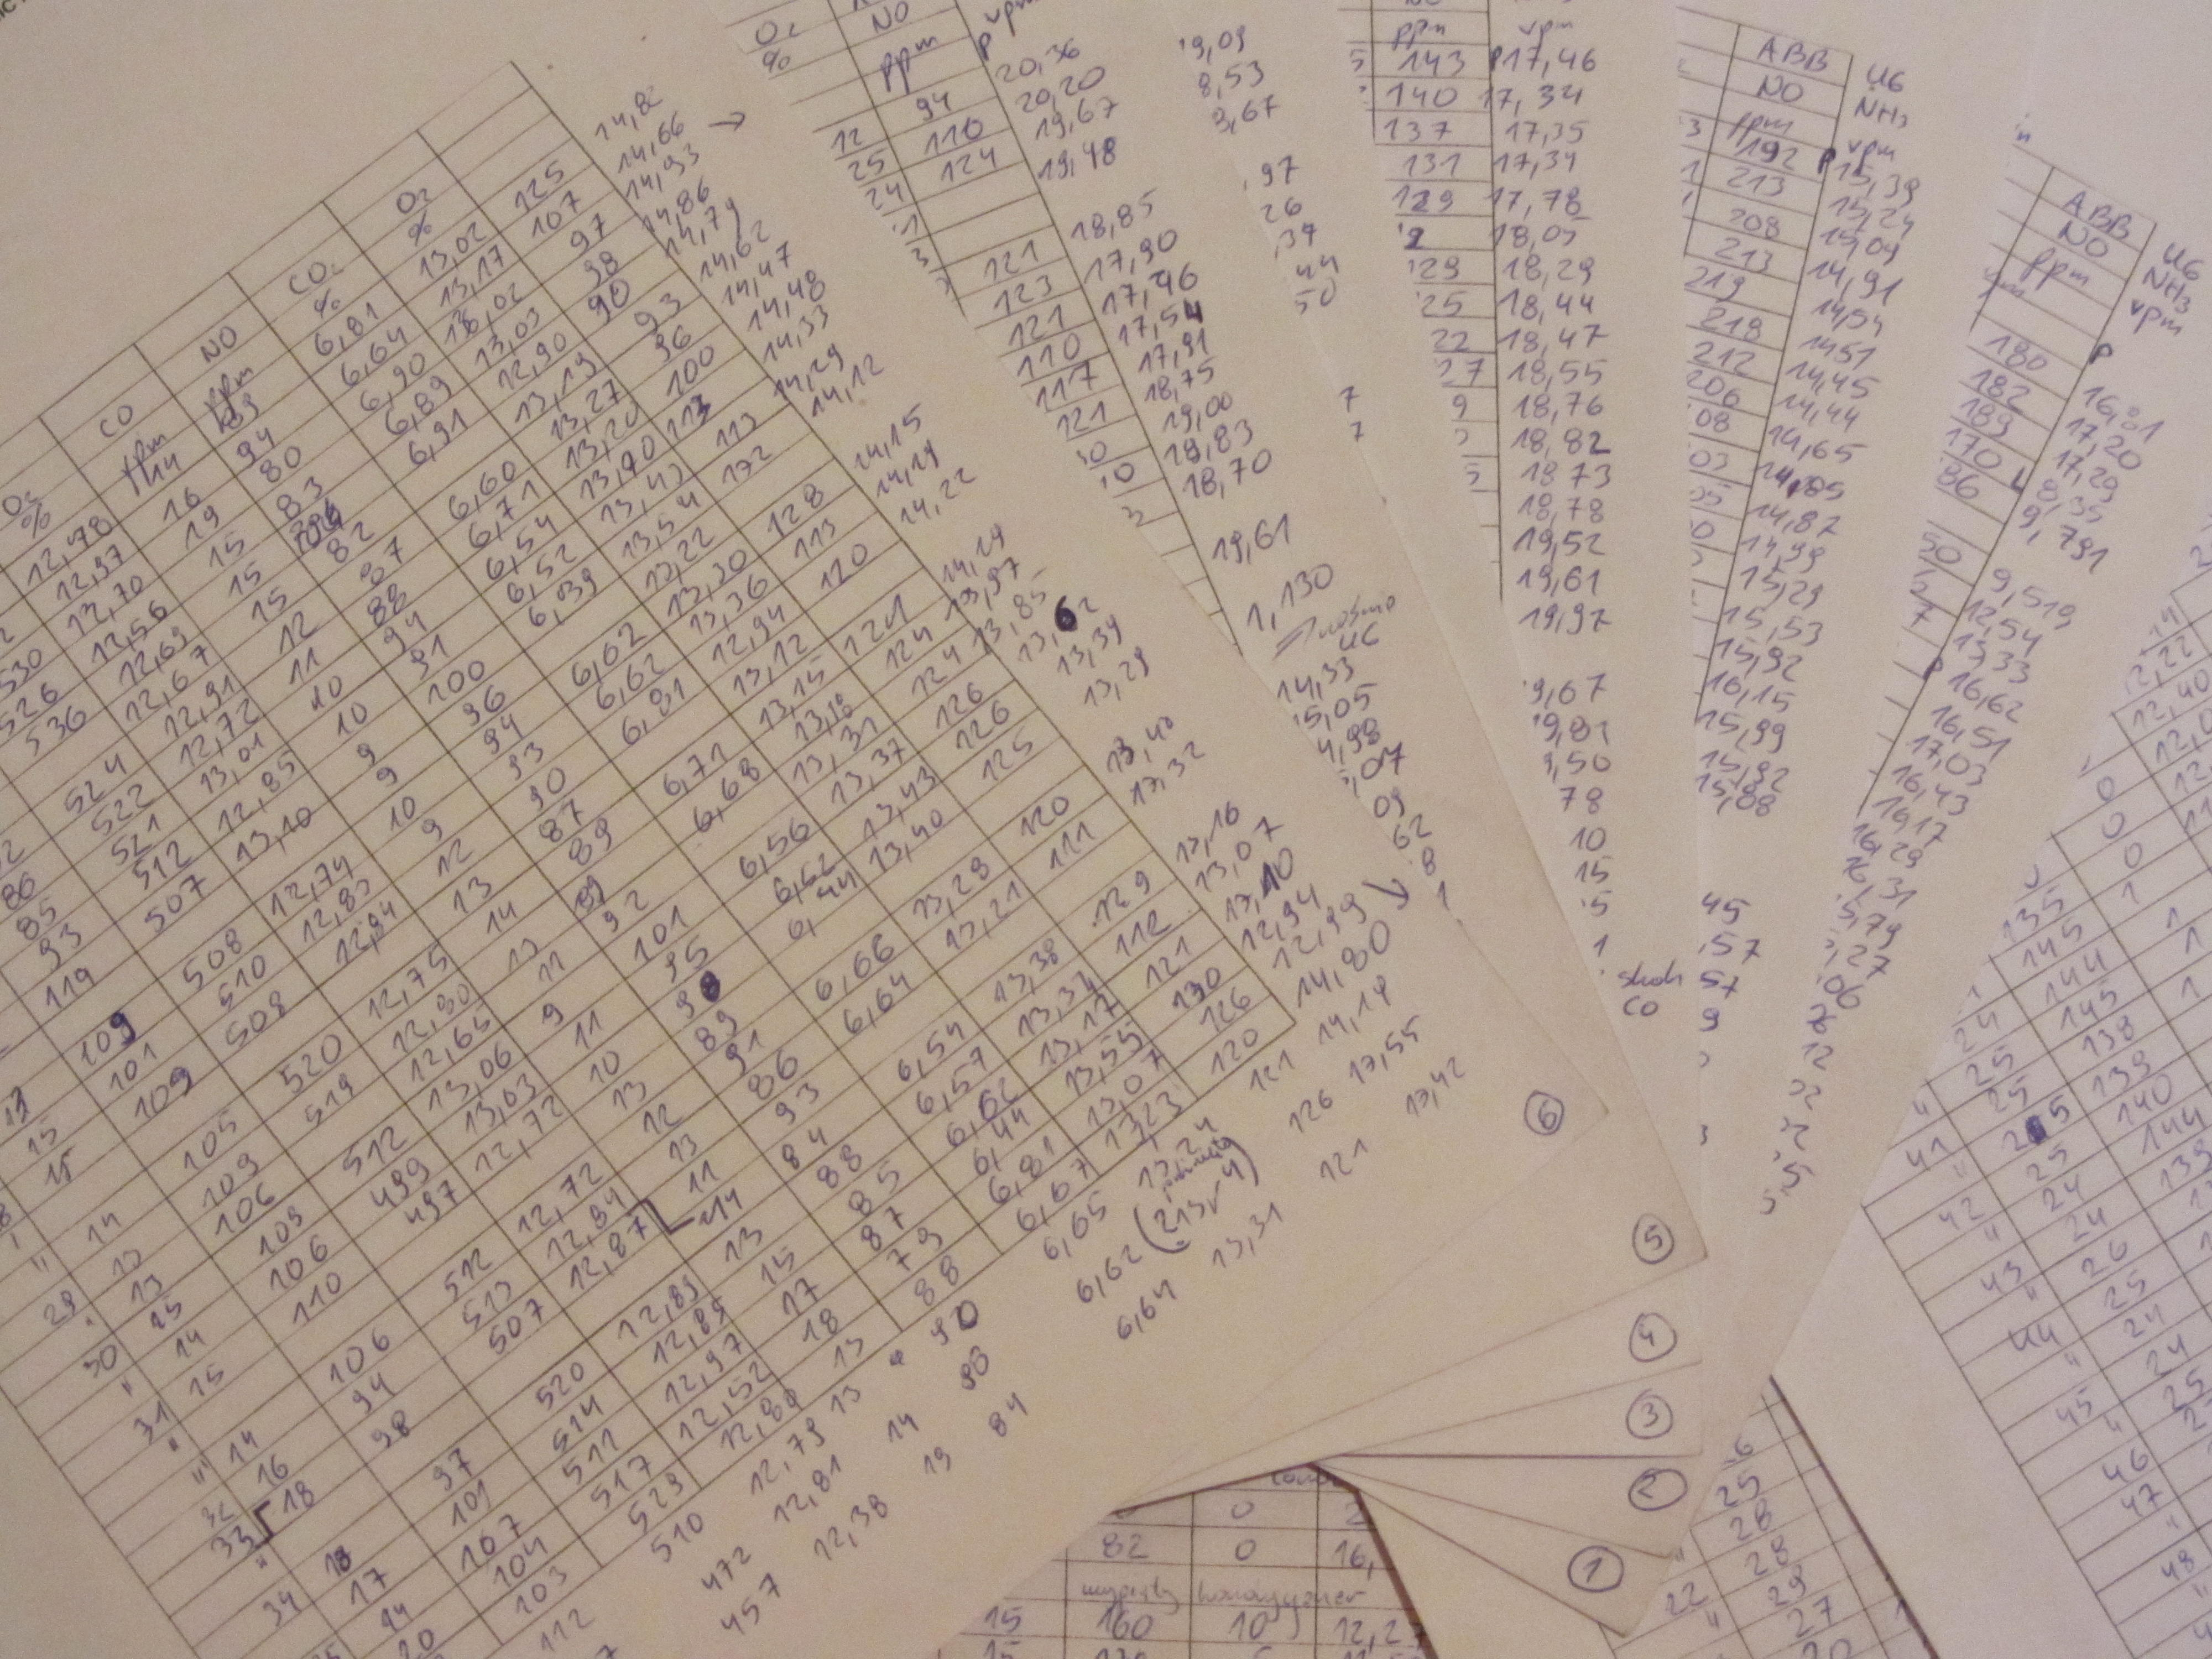
\includegraphics[width=0.99\textheight]{images/IMG_4559}
\end{center}
\end{frame}

%\begin{frame}
%\frametitle{Przykładowa kartka z pomiarem}
%\begin{center}
%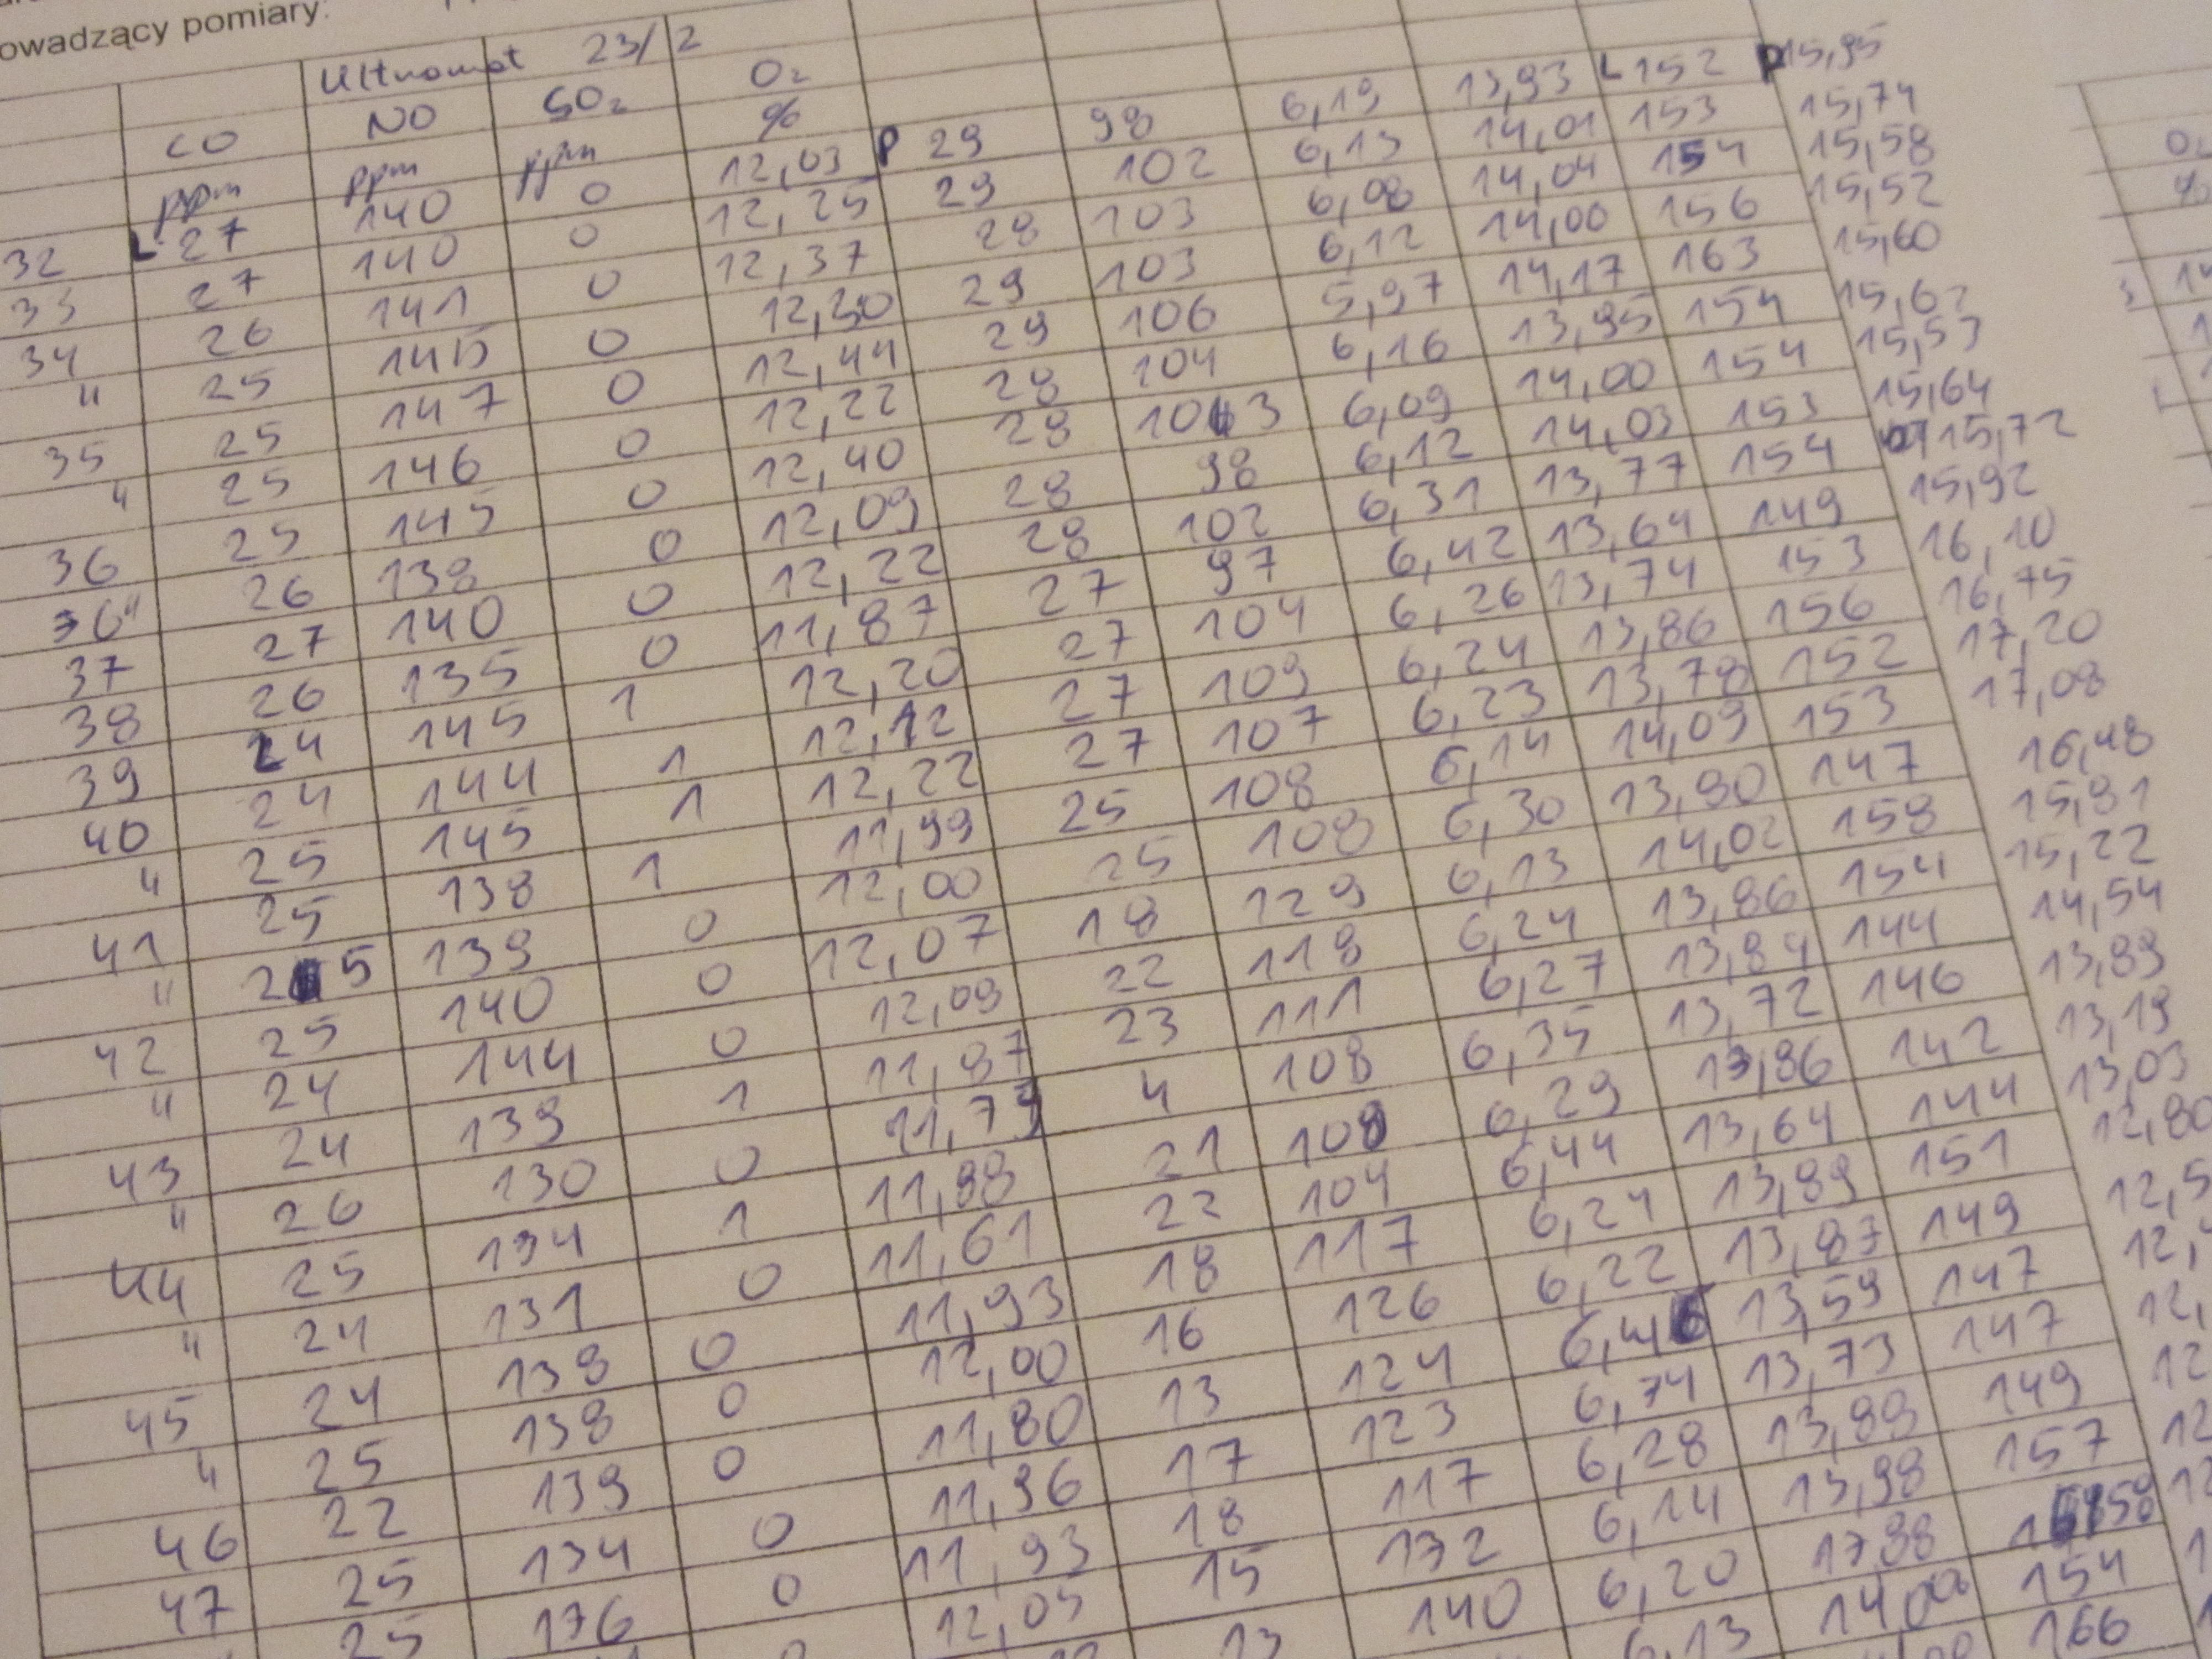
\includegraphics[width=0.99\textheight]{images/IMG_4562}
%\end{center}
%\end{frame}

\begin{frame}
\frametitle{Gas Analyzer - realizacja}
\begin{enumerate}
\item Wykorzystanie protokołu komunikacyjnego ELAN
\item Możliwość podłączenia do 12 analizatorów firmy Siemens:
\begin{itemize}
\item ULTRAMAT 6
\item OXYMAT 6 / OXYMAT 61
\item CALOMAT 6
\item ULTRAMAT 23
\end{itemize}
\item Automatyczny odczyt stanu urządzeń
\item Możliwość archiwizacji pomiarów z dowolnym interwałem czasowym, z~rozdzielczością co sekundę
\item Automatyczne wykrywanie urządzeń i wielkości mierzonych
\item Konfigurowalna precyzja pomiarów (wyświetlanie i raporty)
\item Generowanie raportów do PDF oraz XLS
\item Niskie koszty uruchomienia
\end{enumerate}
\end{frame}

\begin{frame}
\frametitle{Struktura sytemu pomiarowego}
\tikzstyle{background grid}=[draw, black!50,step=.25cm]
	\begin{tikzpicture}[scale=1]%, show background grid]
	\tikzset{
    	mynode/.style={rectangle,rounded corners,draw=black, top color=white, bottom color=yellow!50,very thick, inner sep=0.5em, minimum size=2em, 		text centered, text width=2.8cm},
	    myarrow/.style={->, >=latex', shorten >=1pt, thick},
	    myline/.style={-, =latex', shorten >=1pt, rounded corners, ultra thick},
	    mylabel/.style={text width=7em, text centered} 
	} 
	\node[mynode] (atc) {Konwerter ATC-850};  
	\node [left=of atc] (laptop) {
\includegraphics[width=3cm]{images/laptop}};

	\node[mynode, below=2cm of atc] (device2) {Urządzenie 2};
	\node[mynode, left=of device2] (device1) {Urządzenie 1};  	 	 	
	\node[mynode, right=of device2] (device12) {Urządzenie 12};	

	\draw[myline,blue] (laptop.east) -- ++(-1, 0) -- (atc.west);

	\draw[myline] (atc.south) -- (device1.north); 
	\draw[myline] (atc.south) -- (device2.north); 
	\draw[myline] (atc.south) -- (device12.north); 		
	\draw[myline, dotted] (device2.east) -- (device12.west); 	
    
	\draw [fill=blue!5, thick] (-5, -5) rectangle (1, -4);

    \draw [blue, line width=6] (-4.5,-4.5) -- (-4,-4.5); \node at (-3.5,-4.5) {USB};
    \draw [black, line width=6] (-2,-4.5) -- (-1.5,-4.5); \node at (-0.8,-4.5) {RS-485};
\end{tikzpicture} 
\end{frame}

\begin{frame}
\frametitle{Struktura aplikacji}
\begin{center}
\begin{figure}[htbp]
 \centering
        \tikzstyle{background grid}=[draw, black!50,step=.25cm]
	\begin{tikzpicture}[node distance=2mm, auto]%, show background grid]
	\tikzset{
    	mynode/.style={rectangle,rounded corners,draw=black, top color=white, very thick, inner sep=4mm, 		text centered,font=\footnotesize},
	    myarrow/.style={ <->, shorten >=1pt, line width=1mm},
	    myarrow1/.style={ ->, line width=0.4mm},	    
   	    myarrow2/.style={ ->, shorten >=1mm, line width=0.4mm},
   	    myarrow3/.style={ ->, shorten >=4mm, line width=0.4mm},   	    
	    mylabel/.style={text centered, font=\scriptsize\bfseries} 
	} 
	\node[bottom color=cyan!40, mynode, text width=12cm] (gui) {Graficzny interfejs użytkownika};  
	\node[bottom color=cyan!40, mynode, text width=12cm, text height=2.5cm, below=1cm of gui] (elanNetwork) {Moduł ELAN Network}; 
	\node[bottom color=blue!40, mynode, text width=2cm, below=3cm of gui.173] (a) {Detekcja ramek}; 
	\node[bottom color=blue!40, mynode, text width=2cm, right=of a] (b) {Weryfikacja ramek}; 
	\node[bottom color=blue!40, mynode, text width=2cm, right=of b] (c) {Parsowanie ramek}; 	
	\node[bottom color=blue!40, mynode, text width=2cm, right=of c] (d) {Budowanie migawki}; 
	\node[bottom color=cyan!40, mynode, text width=12cm, below=1cm of elanNetwork] (rxtx) {Biblioteka RXTX}; 
	\node[bottom color=cyan!40, mynode, text width=12cm, below=1cm of rxtx] (conv) {Konwerter RS485 $\Leftrightarrow$ USB};   		
	\node[bottom color=cyan!40, mynode, text width=12cm, below=1cm of conv] (devices) {Urządzenia pomiarowe};	

	\draw[myarrow] (gui.south) -- (elanNetwork.north) node [midway,black] {Przetworzone dane};
	\draw[myarrow] (elanNetwork.south) -- (rxtx.north) node [midway,black] {Odczyt bajtów};	
	\draw[myarrow] (rxtx.south) -- (conv.north) node [midway,black] {USB};	
	\draw[myarrow] (conv.south) -- (devices.north) node [midway,black] {RS485};
	\draw[myarrow1] (a) -- (b);
	\draw[myarrow1] (b) -- (c);
	\draw[myarrow1] (c) -- (d);	
	\draw[myarrow2] (c.north) -- (elanNetwork.north) node [midway,black] {};
	\draw[myarrow3] (d.north) -- (elanNetwork.north) node [midway,black] {};
\end{tikzpicture} 
\caption{Struktura aplikacji.}
\label{appSchema}
\end{figure}
\end{center}
\end{frame}

\begin{frame}
\frametitle{Wykres liczby odebranych ramek z danymi pomiarowymi}
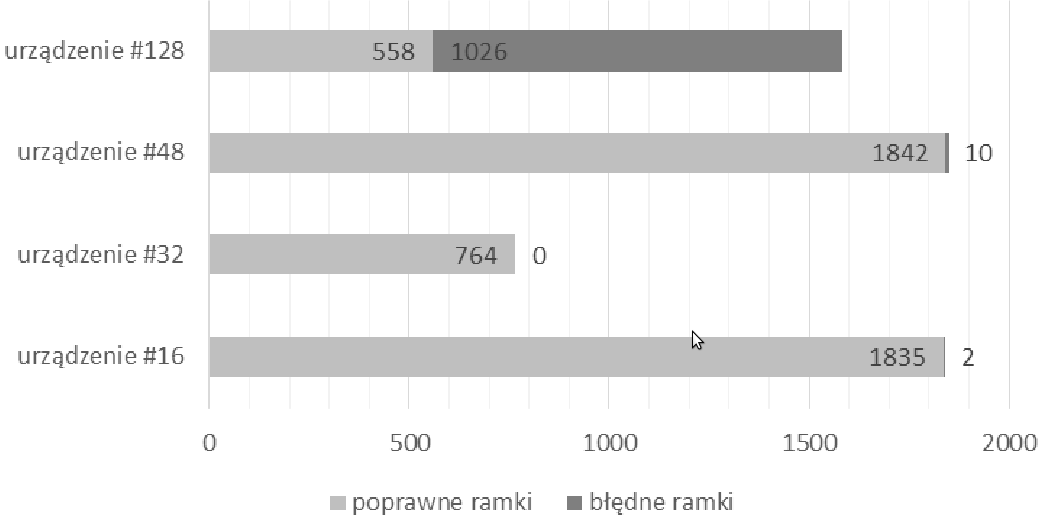
\includegraphics[width=0.99\textwidth]{images/wykres}
\end{frame}

\begin{frame}
\frametitle{Średni interwał czasu pomiędzy kolejnymi transmisjami poprawnych ramek pomiarowych z analizatorów}
\begin{center}
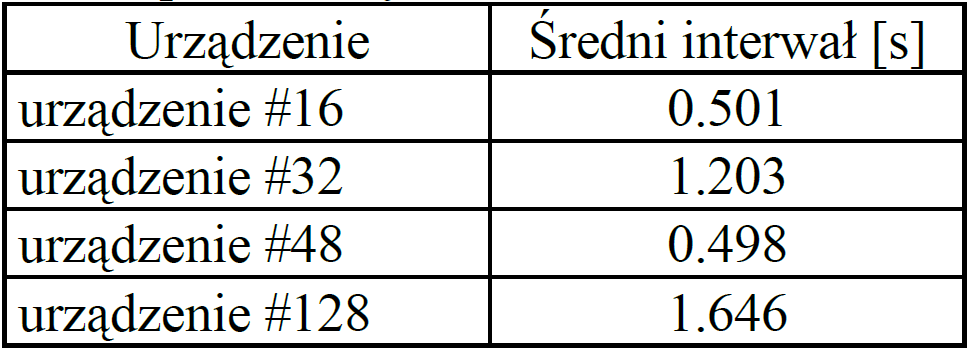
\includegraphics[width=0.80\textwidth]{images/timeToNextFrame.png}
\end{center}
\end{frame}

\begin{frame}
\frametitle{ELAN Network zasada działania buforów}
\tikzstyle{background grid}=[draw, black!50,step=.25cm]
\newcounter{wavenum}
\newcounter{iter}

\setlength{\unitlength}{1cm}

% advance clock one cycle, not to be called directly
\newcommand*{\clki}[1]{
  \draw[white] (t_cur) -- ++(#1,0) node[time] (t_cur) {};
}

\newcommand*{\bitvector}[3]{
  \draw[fill=#3] (t_cur) -- ++( .1, .3) -- ++(#2-.2,0) -- ++(.1, -.3)
                         -- ++(-.1,-.3) -- ++(.2-#2,0) -- cycle;
  \path (t_cur) -- node[anchor=mid] {#1} ++(#2,0) node[time] (t_cur) {};
}

% \known{val}{length}
\newcommand*{\known}[2][]{
    \bitvector{#1}{#2}{white}
}

% \unknown{length}
\newcommand*{\unknown}[2][]{
    \bitvector{#1}{#2}{black!30}
}

% \bit{1 or 0}{length}
\newcommand*{\bit}[2]{
  \draw (t_cur) -- ++(0,.6*#1-.3) -- ++(#2,0) -- ++(0,.3-.6*#1)
    node[time] (t_cur) {};
}
\newcommand*{\lbl}[2]{
 \path (t_cur) -- node[time] {} ++(#2-.2,0) node[anchor=mid] (t_cur) {#1} ++(.2,0) node[time] (t_cur) {};
}

% \nextwave{name}
\newcommand{\nextwave}[1]{
  \path (0,\value{wavenum}) node[left=0.5cm] {#1} node[time] (t_cur) {};
  \addtocounter{wavenum}{-1}
}

\newcommand{\nr}{
	$\Rightarrow$
}

\newcommand{\ur}{
	$\circlearrowleft$
}

% \clk{name}{period}
\newcommand{\clk}[2]{
    \nextwave{#1}
    \FPeval{\res}{(\wavewidth+1)/#2}
    \FPeval{\reshalf}{#2/2}
    \foreach \t in {1,2,...,\res}{
        \bit{\reshalf}{1}
        \bit{\reshalf}{0}
    }
}
    
% \begin{wave}[clkname]{num_waves}{clock_cycles}
\newenvironment{wave}[3][]{
  \begin{tikzpicture}[draw=black, yscale=.7,xscale=1]%, show background grid]
    \tikzstyle{time}=[coordinate]
    \setlength{\unitlength}{1cm}
    \def\wavewidth{#3}
    \setcounter{wavenum}{0}
    \nextwave{#1}
    \def\myarray{1,5,1}
    %\foreach \t in {0,1,...,\wavewidth}{
    \foreach \i / \x in {0/1.5, 1/2, 2/1.25, 3/2.5, 4/.75, 5/1, 6/1.75} {
      \draw[dotted] (t_cur) +(0,.1) node[above] {$t_\i$} -- ++(0,.4-#2);
      \clki{\x};
    }
    \draw[->, >=latex', shorten >=1pt, thick] (-.4,-3.5) -- (-.4,0);
    \draw[->, >=latex', shorten >=1pt, thick] (-.4,-3.5) -- (10,-3.5);
}
{\end{tikzpicture}}

\begin{wave}{4}{15}
 \nextwave{Bufor 1}  \lbl{\nr}{0} \known{.5} \lbl{}{1} \unknown{.5} \lbl{\ur}{1.5} \unknown{.5} \lbl{}{.75} \unknown{.5} \lbl{}{2} \unknown{.5} \lbl{}{1.25} \known{.5}
 \nextwave{Bufor 2}  \known{.5} \lbl{}{1} \known{.5} \lbl{}{1.5} \known{.5} \lbl{\nr}{.75} \known{.5} \lbl{}{2} \unknown{.5} \lbl{\nr}{1.25} \known{.5}
 \nextwave{Bufor 3} \known{.5} \lbl{\nr}{1} \known{.5}	\lbl{}{1.5} \unknown{.5} \lbl{}{.75} \unknown{.5} \lbl{\ur}{2} \unknown{.5} \lbl{}{1.25} \known{.5}
\end{wave}

$t_0$ -- nadejście pomiaru z urządzenia 1 \\
$t_1$ -- nadejście pomiaru z urządzenia 3 \\
$t_2$ -- nadejście pomiaru z urządzenia 1 \\
$t_3$ -- nadejście pomiaru z urządzenia 2 \\
$t_4$ -- nadejście pomiaru z urządzenia 3 \\
$t_5$ -- Migawka, czyli zapis wszystkich buforów do bazy \\
$t_6$ -- nadejście pomiaru z urządzenia 2 
\end{frame}

\begin{frame}
\frametitle{Wyniki pomiarów czasów otrzymania potwierdzenia i odpowiedzi analizatorów na komendę – pomiar z zastosowaniem zestawu ewaluacyjnego}
\begin{center}
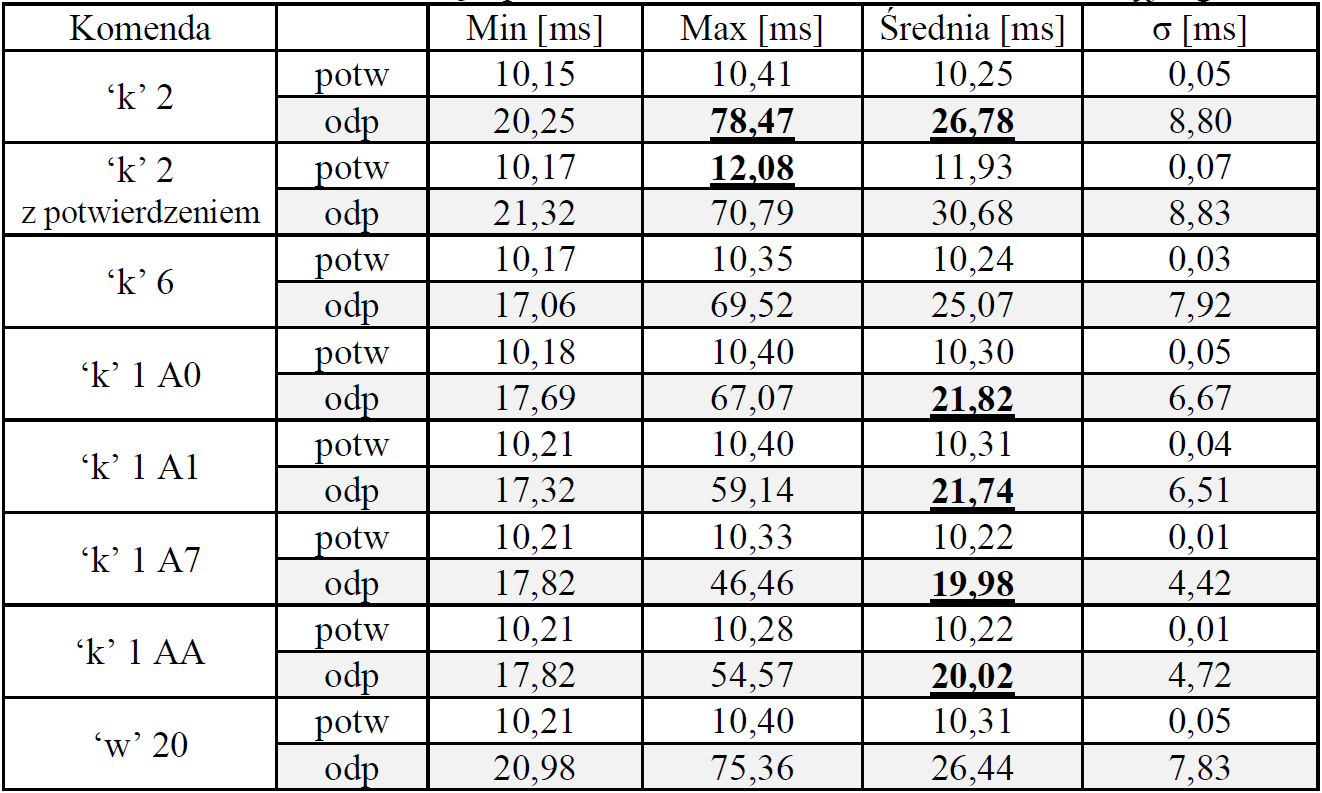
\includegraphics[width=0.80\textwidth]{images/tabela1.png}
\end{center}
\end{frame}

\begin{frame}
\frametitle{Wyniki pomiarów czasów otrzymania potwierdzenia i odpowiedzi analizatorów na komendę – pomiar z zastosowaniem komputera przenośnego}
\begin{center}
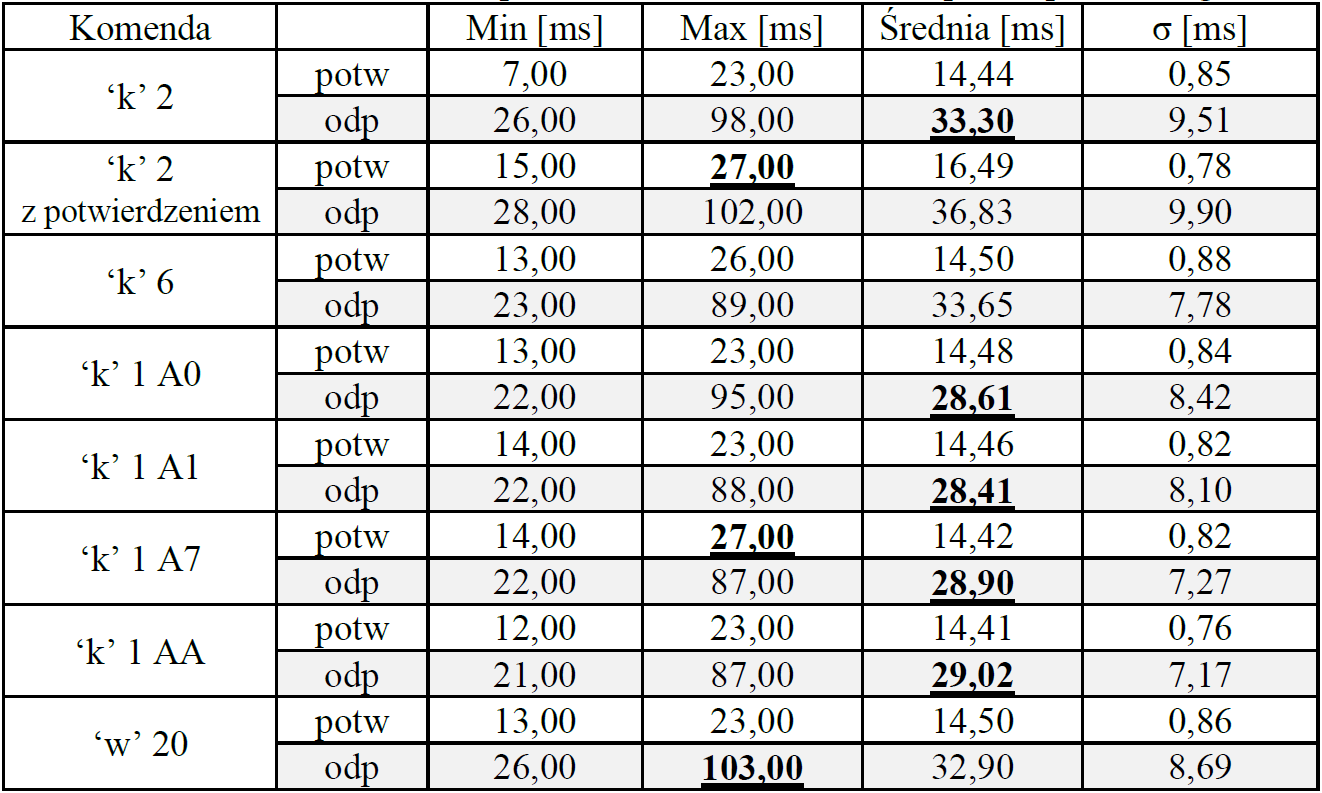
\includegraphics[width=0.80\textwidth]{images/tabela2.png}
\end{center}
\end{frame}

\begin{frame}
\frametitle{Wykres czasów otrzymania potwierdzenia oraz odpowiedzi na komendę 'k'2}
\begin{center}
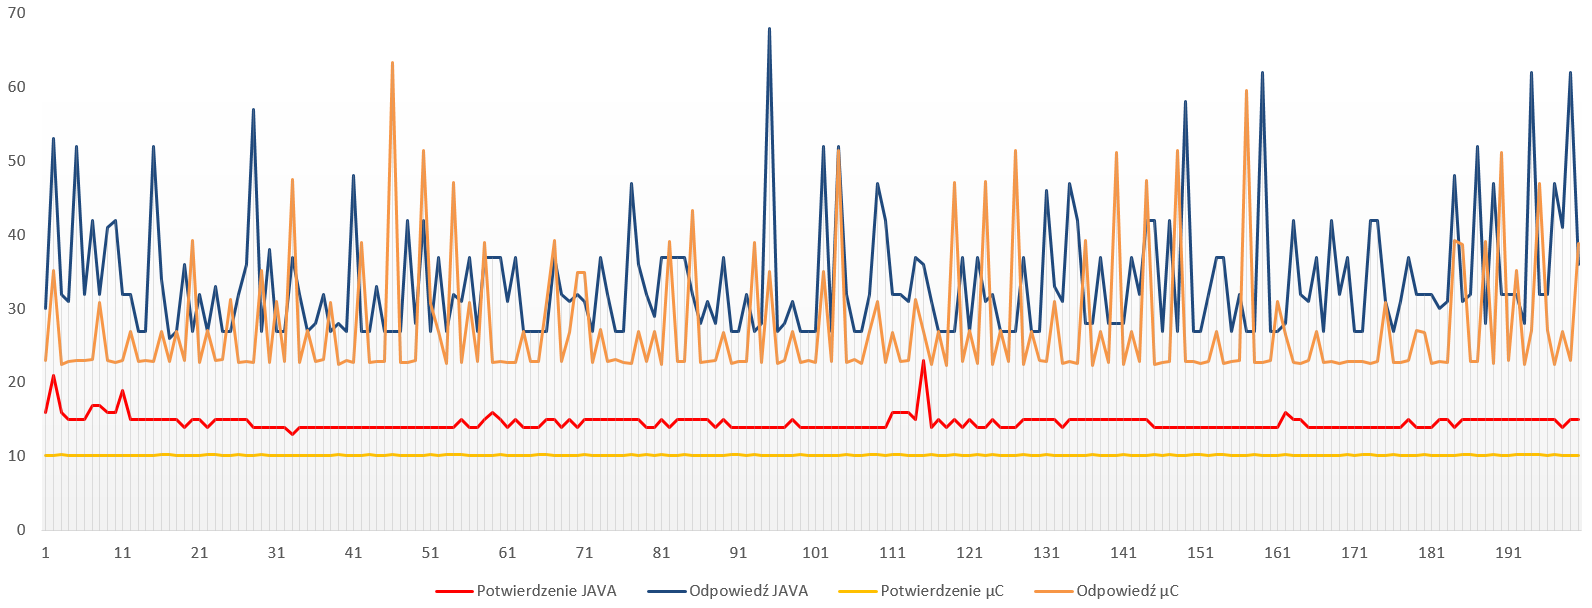
\includegraphics[width=0.90\textwidth]{images/wykres_k2.png}
\end{center}
\end{frame}

\begin{frame}
\frametitle{Podgląd sieci}
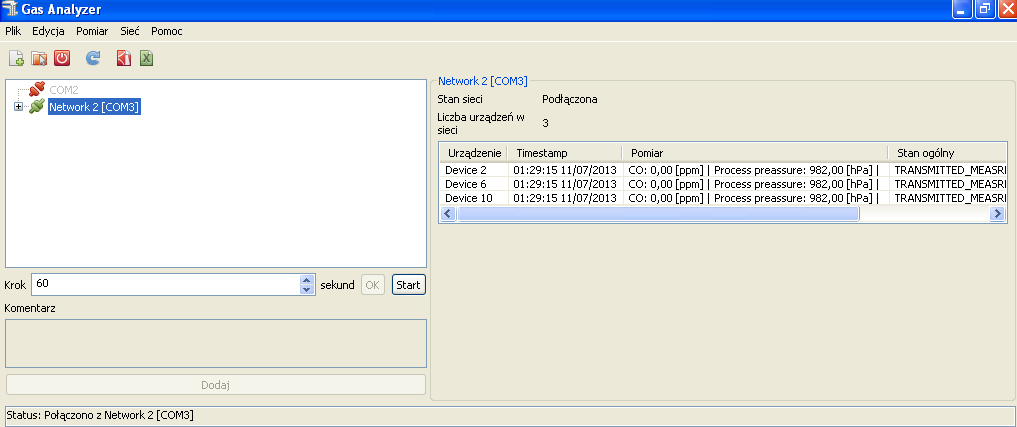
\includegraphics[width=0.99\textwidth]{images/detailNetworkW}
\end{frame}

\begin{frame}
\frametitle{Podgląd urządzenia}
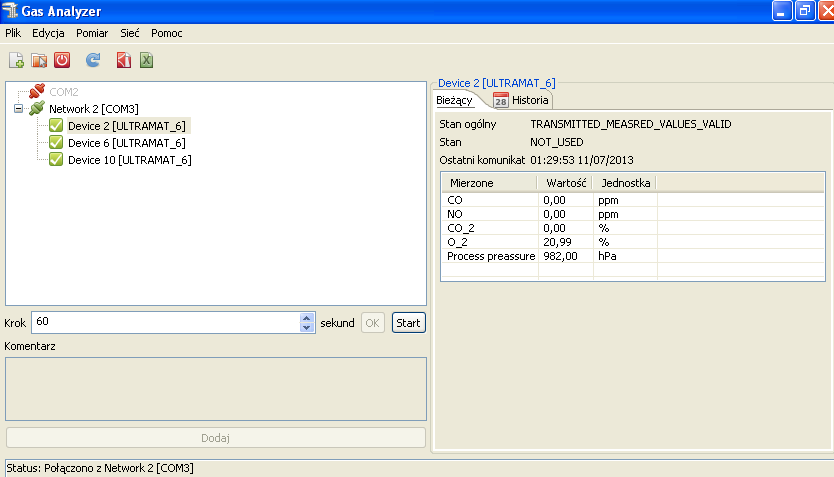
\includegraphics[width=0.99\textwidth]{images/detailDeviceW}
\end{frame}

\begin{frame}
\frametitle{Przykładowy raport PDF}
\begin{center}

\includegraphics[width=0.99\textwidth]{images/pdf}
\end{center}
\end{frame}

\begin{frame}
\frametitle{Przykładowy raport XLS}
\begin{center}
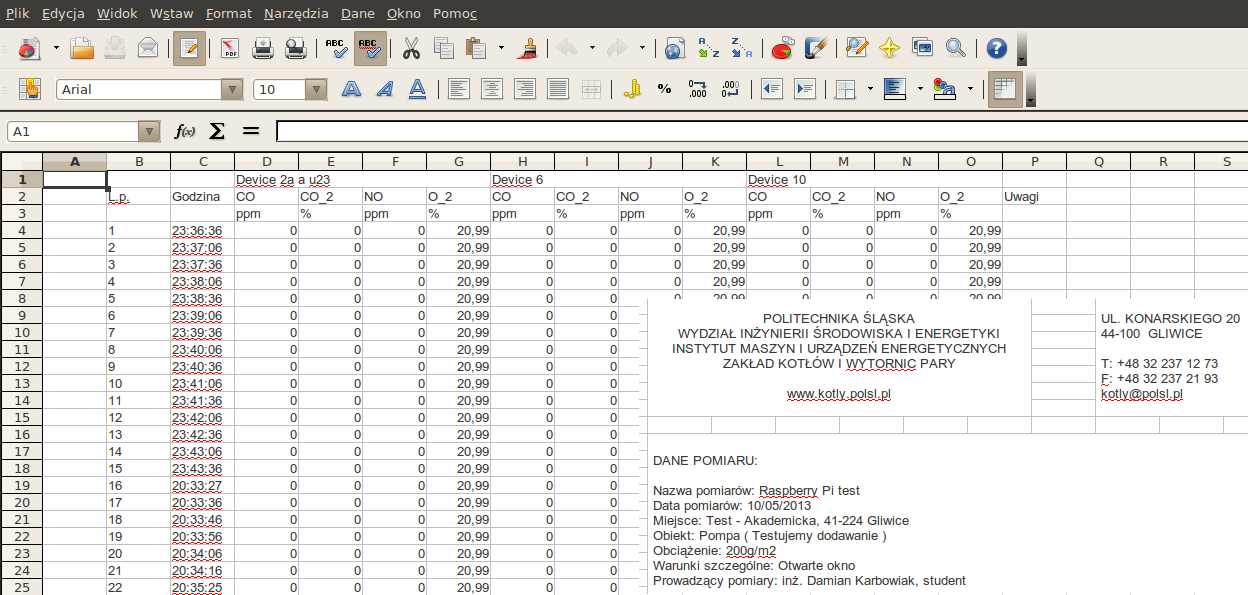
\includegraphics[width=0.99\textwidth]{images/xls}
\end{center}
\end{frame}

%\section{Podsumowanie}
\begin{frame}
\frametitle{Testy w warunkach laboratoryjnych}
\begin{center}
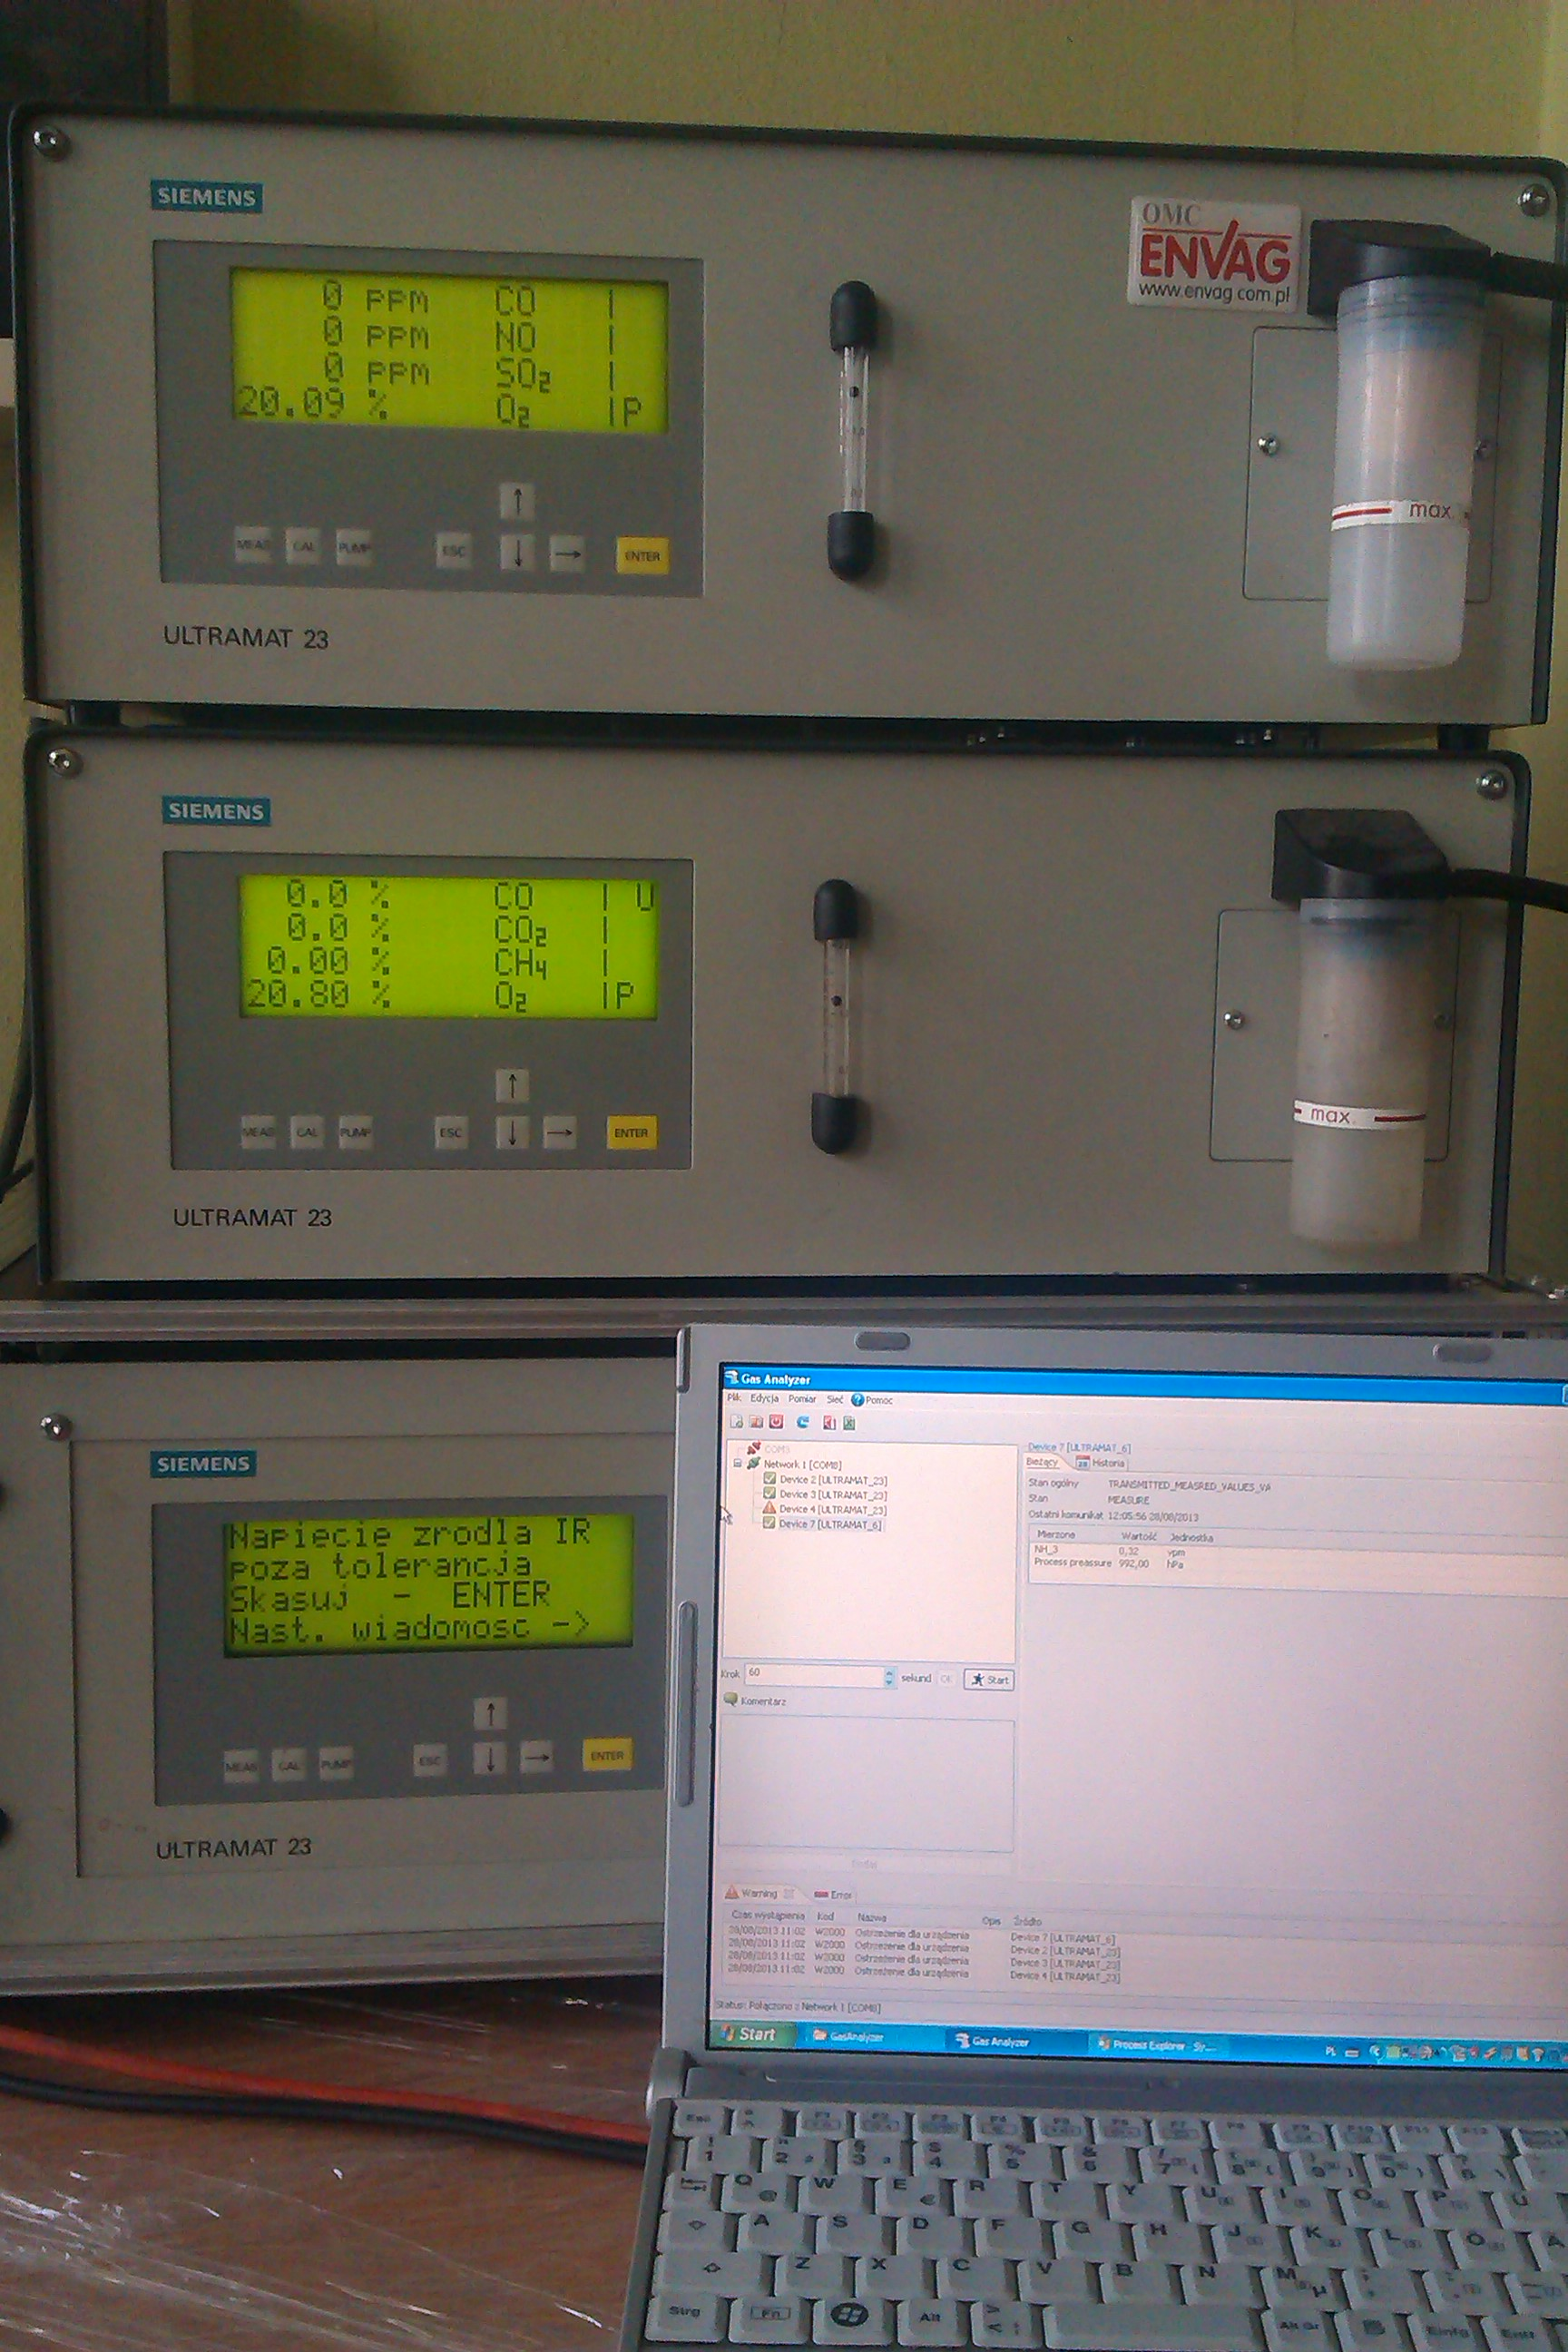
\includegraphics[height=0.8\textheight]{images/lab1}
\end{center}
\end{frame}

\begin{frame}
\frametitle{Testy w warunkach laboratoryjnych}
\begin{center}
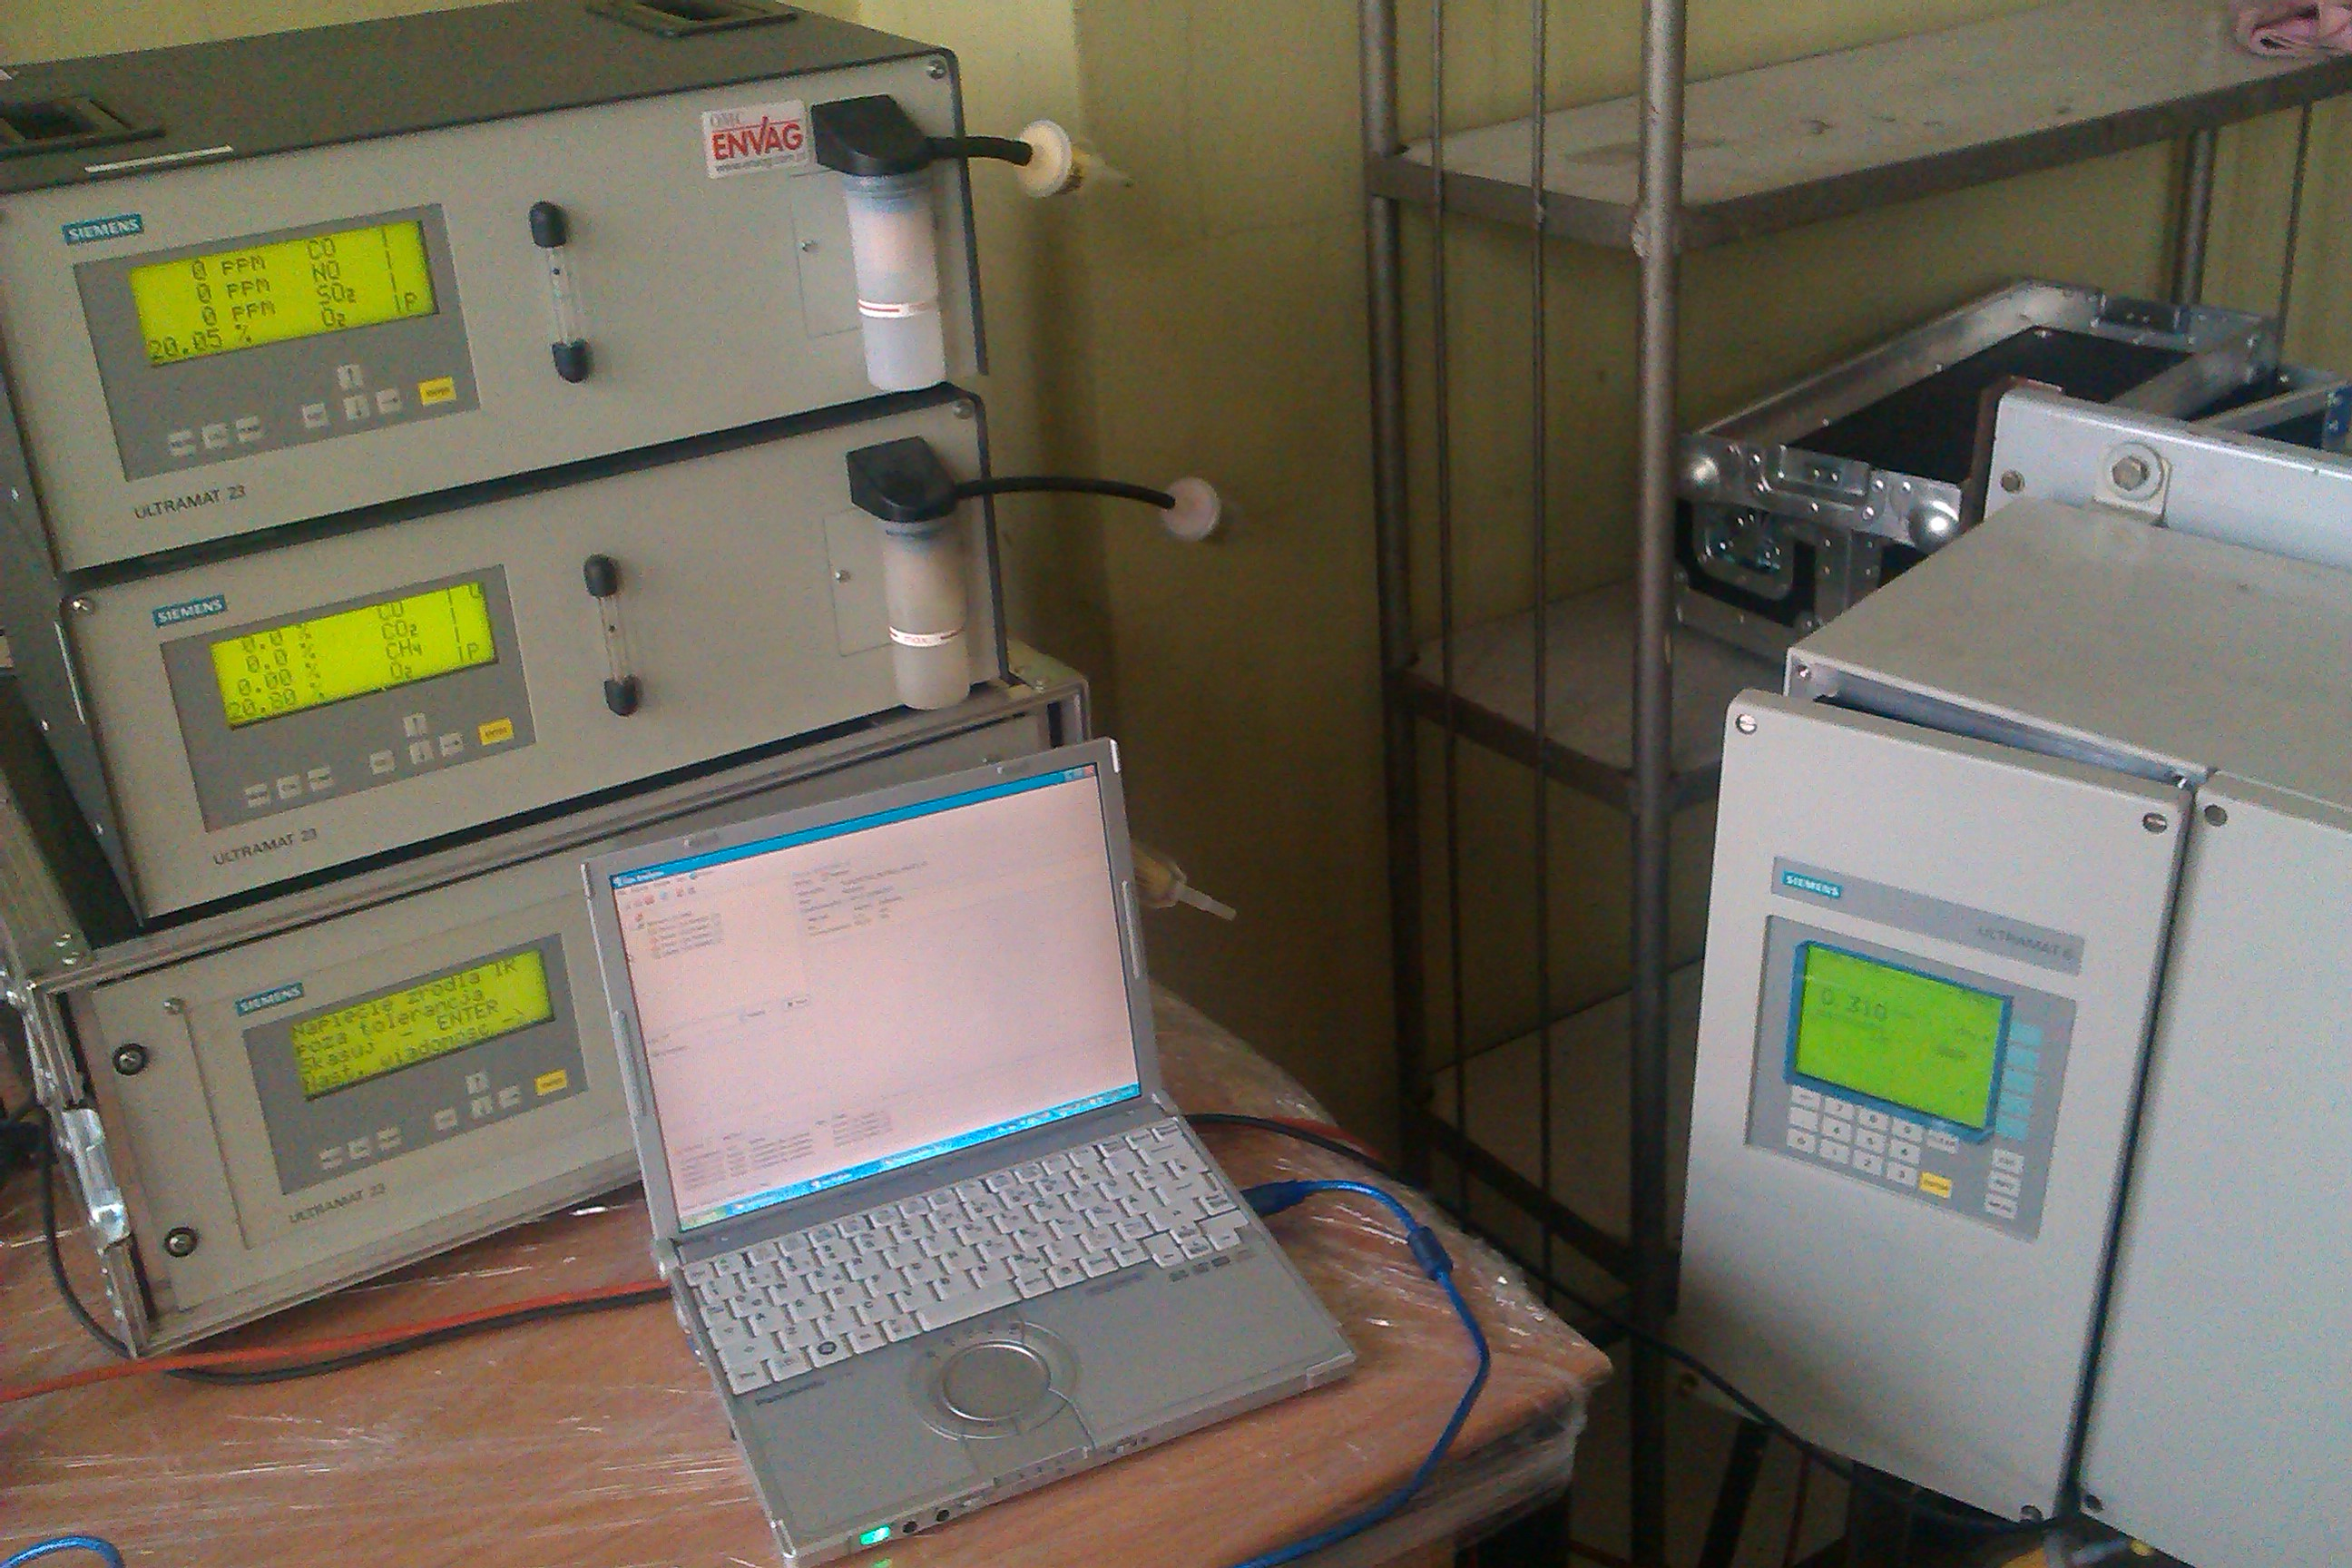
\includegraphics[width=0.9\textwidth]{images/lab2}
\end{center}
\end{frame}

\begin{frame}
\frametitle{Testy w warunkach przemysłowych}
\begin{itemize}
\setlength{\itemsep}{5pt}
\setlength{\parskip}{5pt}
\setlength{\parsep}{5pt}
\item Elektrociepłownia Marcel Sp. z o.o.; Radlin marzec 2014
\item Zespół Elektrociepłowni Wrocławskich KOGENERACJA S.A.; Wrocław marzec 2014
\item ENERGA Elektrownie Ostrołęka S.A.; Ostrołęka grudzień 2013
\item Laboratorium Procesów Kotłowych ZKiWP Instytutu Maszyn i Urządzeń Energetycznych Politechnika Śląska; Gliwice na co dzień
\end{itemize}
\end{frame}

\begin{frame}
\frametitle{Perspektywy rozwoju}
\begin{itemize}
\setlength{\itemsep}{5pt}
\setlength{\parskip}{5pt}
\setlength{\parsep}{5pt}
\item Generowanie przebiegów wybranych wartości
\item Zmiana modelu wymiany danych
\item Poprawa parametrów czasowych
\item Implementacja oprogramowania analitycznego
\item Integracja wielu standardów komunikacyjnych
\item Utworzenie zintegrowanego systemu pomiarowego
\end{itemize}
\end{frame}

\begin{frame}
\frametitle{Wnioski}
\begin{itemize}
\setlength{\itemsep}{5pt}
\setlength{\parskip}{5pt}
\setlength{\parsep}{5pt}
\item Brak determinizmu (CSMA$\backslash$CD)
\item Wystarczające (statystycznie) parametry czasowe
\item Niski koszt rozwiązania
\item Przenośność i łatwość rozbudowy aplikacji
\end{itemize}
\end{frame}

\begin{frame}
\frametitle{Podsumowanie oraz pytania}
Dziękujemy za uwagę.
\\\vspace{2cm}
Czas na pytania.
\\\vspace{2cm}
mgr inż. Damian Karbowiak -- Damian.Karbowiak@polsl.pl
\\\vspace{2mm}
mgr inż. Grzegorz Powała  -- Grzegorz.Powala@polsl.pl
\end{frame}

\end{document}